\section{Modeling}
\label{sec:modeling}

All models in this section are trained on the 17 training records and compared on the 5 validation records of Table~\ref{tab:records}. DS2 is not read until Section~\ref{sec:evaluation}. Everything runs from \texttt{notebooks/MODELING.ipynb}, which calls the package \texttt{ecg} (\texttt{src/ecg/datasets}, \texttt{models}, \texttt{training}); the settings are in \texttt{configs/model.yaml}, \texttt{baselines.yaml} and \texttt{sweep.yaml}, and every training run is one row of \texttt{results/experiments.csv}.

\subsection{Baseline}
\label{sec:baseline}

Two classical models serve as reference points. Both receive the flattened beat window (the same 256 values the first CNN sees) plus the three RR-interval features of Section~\ref{sec:beat-extraction}: the time since the previous beat, the time to the next beat, and the ratio of the first to the local mean. The RR features are the standard hand-made timing cue that separates an early S beat from an N beat, so on timing the baselines know more than a single-beat CNN.

\begin{itemize}[nosep]
  \item \textbf{Logistic regression} on standardised features, with balanced class weights.
  \item \textbf{Random forest} with 200 trees, at least two beats per leaf, and balanced class weights.
\end{itemize}

\begin{table}[H]
  \centering
  \caption{Baselines on the validation records. Both see the flattened beat plus the three RR features. Params: coefficients for the logistic regression, tree nodes for the forest.}
  \label{tab:baselines}
  \rowcolors{2}{white}{rowtint}
  \begin{tabularx}{\linewidth}{lRRRRRRR}
    \rowcolor{primaryblue}
    \hd{Model} & \hd{Params} & \hd{Accuracy} & \hd{Macro-F1} & \hd{S prec.} & \hd{S recall} & \hd{V recall} & \hd{F recall} \\
    Logistic regression & 1\,040 & 0.894 & 0.462 & 0.254 & 0.319 & 0.535 & 0.125 \\
    Random forest & 150\,574 & 0.933 & 0.430 & 0.933 & 0.043 & 0.529 & 0.000 \\
    \bottomrule
  \end{tabularx}
\end{table}


Table~\ref{tab:baselines} shows the validation scores. The logistic regression reaches a macro-F1 of 0.46, the random forest 0.43. The forest is more accurate (0.93) but finds almost no S beats (recall 0.04) and no F beats, even though it has the RR features: with 90\,\% normal beats, the trees still favour the majority class on unseen records. The logistic regression trades accuracy for a better S recall (0.32). Both are far below the success criterion of 0.70, which sets the bar the CNN has to clear.

\subsection{Proposed Edge Model}
\label{sec:edge-model}

The final network is a 1D CNN with four fused convolution blocks and one fully connected output layer (Table~\ref{tab:architecture}). It takes one channel of 512 samples, the wide beat window of Section~\ref{sec:beat-extraction}, scaled to $[-1, 1)$.

\begin{table}[H]
  \centering
  \caption{Layers of the final CNN as the accelerator runs them. Each row is one fused layer; the pool, when present, runs before the convolution.}
  \label{tab:architecture}
  \rowcolors{2}{white}{rowtint}
  \begin{tabularx}{\linewidth}{llYlr}
    \rowcolor{primaryblue}
    \hd{Layer} & \hd{Input} & \hd{Operation} & \hd{Output} & \hd{Parameters} \\
    conv1 & 1 x 512 & Conv1d k=5 p=2, ReLU & 16 x 512 & 96 \\
    conv2 & 16 x 512 & MaxPool 2, Conv1d k=5 p=2, ReLU & 32 x 256 & 2\,592 \\
    conv3 & 32 x 256 & MaxPool 4, Conv1d k=3 p=1, ReLU & 64 x 64 & 6\,208 \\
    conv4 & 64 x 64 & MaxPool 4, Conv1d k=3 p=1, ReLU & 64 x 16 & 12\,352 \\
    fc & 1024 (flattened) & Linear & 4 & 4\,100 \\
    Total &  &  &  & 25\,348 \\
    \bottomrule
  \end{tabularx}
\end{table}


Each block is one accelerator layer: an optional max-pool, a convolution with zero padding, and a ReLU. The pools halve the length after the first block, then quarter it twice, so the 512 input samples become 16 positions with 64 channels, which are flattened into 1\,024 values for the output layer. Kernel lengths 5 and 3 with paddings 2 and 1 keep the length through each convolution. BatchNorm after every convolution (352 extra parameters) helped the wide-window model train in the sweep; it is folded into the convolution weights before quantisation and is absent from the deployed network, which has 25\,348 weights and biases.

The architecture suits the accelerator. It uses only operations the MAX78002 executes natively (1D convolution with kernels up to 9, pooling fused into the convolution, ReLU, one small fully connected layer), so no operator falls back to the Cortex-M4 core. Its 25\,348 parameters are about 25\,kB in INT8, 1\,\% of the chip's weight memory and a quarter of the 100\,000-parameter budget of Section~\ref{sec:success-criteria}. The largest intermediate tensor is $16 \times 512$ bytes, and the input is a fixed-size tensor, which is what the accelerator's data memory expects. Transformers, recurrent layers, attention and large residual networks were not considered, because they either use unsupported operators or do not fit; the course text excludes them for the same reasons.

\subsection{Training Configuration}
\label{sec:training-config}

\begin{table}[H]
  \centering
  \caption{Training configuration of the final model.}
  \label{tab:training-config}
  \rowcolors{2}{white}{rowtint}
  \begin{tabularx}{\linewidth}{lY}
    \rowcolor{primaryblue}
    \hd{Setting} & \hd{Value} \\
    Input & 1 $\times$ 512 samples, scaled to $[-1, 1)$ \\
    Optimizer & Adam, weight decay 0 \\
    Learning rate & 0.001, cosine decay over 60 epochs \\
    Batch size & 128 \\
    Epochs & at most 60; stopped after 28, best epoch 18 \\
    Loss & cross-entropy \\
    Class weighting & none \\
    Oversampling & sampler weight (1 / class frequency) to the power 0.5 \\
    Early stopping & patience 10 epochs on validation macro-F1 \\
    Augmentation & amplitude scaling [0.8, 1.2], time shift $\pm$5 samples, baseline wander up to 0.3, Gaussian noise $\sigma$ = 0.02 \\
    Dropout & 0.000 \\
    Random seed & 42 \\
    \bottomrule
  \end{tabularx}
\end{table}


The loss is plain cross-entropy; the class imbalance is handled by the sampler, which draws each beat with probability proportional to the inverse square root of its class frequency, so about a third of every batch is S, V or F while N still dominates. Section~\ref{sec:model-selection} explains why this was preferred to class weights. Augmentation is applied on the fly to training beats only: amplitude scaling, a time shift of up to five samples, a slow sine as baseline wander, and light Gaussian noise. The learning rate follows a cosine decay and early stopping keeps the epoch with the best validation macro-F1 (Figure~\ref{fig:learning-curve}). All runs use seed 42 for Python, NumPy and PyTorch.

\begin{figure}[H]
  \centering
  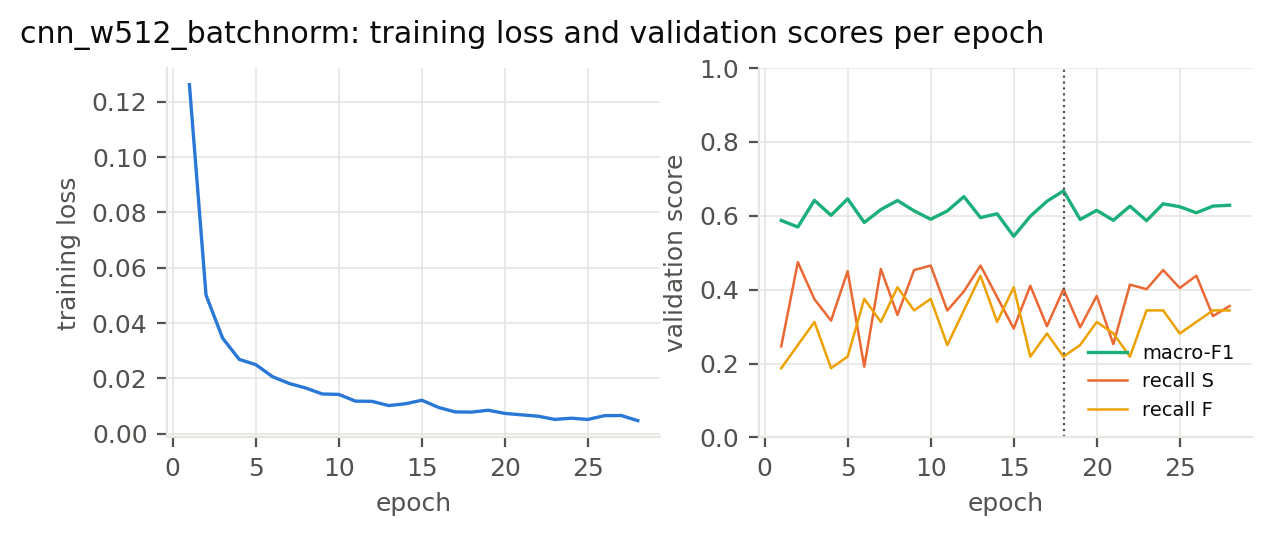
\includegraphics[width=\linewidth]{learning_curve.png}
  \caption{The final run: training loss (left) and validation macro-F1 and S/F recall per epoch (right). The dotted line marks the epoch whose weights were kept.}
  \label{fig:learning-curve}
\end{figure}

\subsection{Model Selection}
\label{sec:model-selection}

Model selection was a staged sweep (\texttt{configs/sweep.yaml}), always scored by macro-F1 on the validation records. Each stage starts from the best run so far, so a later stage only has to vary what it is about. Table~\ref{tab:model-selection} lists every run.

\begin{table}[H]
  \centering
  \caption{Model-selection sweep on the validation records, best first. Window is the input length in samples.}
  \label{tab:model-selection}
  \rowcolors{2}{white}{rowtint}
  \begin{tabularx}{\linewidth}{lRRRRRRRRRR}
    \rowcolor{primaryblue}
    \hd{Run} & \hd{Stage} & \hd{Window} & \hd{Params} & \hd{Best epoch} & \hd{Accuracy} & \hd{Macro-F1} & \hd{S prec.} & \hd{S recall} & \hd{V recall} & \hd{F recall} \\
    cnn\_w512\_batchnorm & 3 & 512 & 25\,700 & 18 & 0.965 & 0.667 & 0.846 & 0.401 & 0.840 & 0.219 \\
    cnn\_w512\_mild\_balance & 3 & 512 & 25\,348 & 35 & 0.951 & 0.614 & 0.616 & 0.444 & 0.802 & 0.281 \\
    cnn\_w512\_large & 3 & 512 & 39\,300 & 28 & 0.949 & 0.613 & 0.478 & 0.429 & 0.848 & 0.344 \\
    cnn\_w512\_small & 3 & 512 & 7\,428 & 6 & 0.954 & 0.598 & 0.567 & 0.362 & 0.835 & 0.219 \\
    cnn\_w512\_no\_aug & 3 & 512 & 25\,348 & 9 & 0.946 & 0.596 & 0.454 & 0.453 & 0.788 & 0.219 \\
    cnn\_w512 & 2 & 512 & 25\,348 & 4 & 0.947 & 0.591 & 0.472 & 0.465 & 0.736 & 0.156 \\
    cnn\_oversample\_only & 1 & 256 & 25\,348 & 8 & 0.955 & 0.569 & 0.441 & 0.237 & 0.929 & 0.156 \\
    cnn\_mild\_balance & 1 & 256 & 25\,348 & 6 & 0.946 & 0.564 & 0.471 & 0.219 & 0.923 & 0.312 \\
    cnn\_no\_aug & 2 & 256 & 25\,348 & 5 & 0.938 & 0.562 & 0.544 & 0.280 & 0.833 & 0.250 \\
    cnn\_batchnorm & 2 & 256 & 25\,700 & 20 & 0.951 & 0.557 & 0.416 & 0.286 & 0.920 & 0.031 \\
    cnn\_small & 2 & 256 & 7\,428 & 8 & 0.953 & 0.555 & 0.508 & 0.195 & 0.901 & 0.156 \\
    cnn\_large & 2 & 256 & 39\,300 & 22 & 0.943 & 0.554 & 0.249 & 0.222 & 0.961 & 0.156 \\
    cnn\_regularised & 2 & 256 & 25\,348 & 10 & 0.953 & 0.550 & 0.480 & 0.182 & 0.932 & 0.094 \\
    cnn\_weights\_only & 1 & 256 & 25\,348 & 7 & 0.950 & 0.548 & 0.583 & 0.182 & 0.905 & 0.156 \\
    cnn\_focal & 1 & 256 & 25\,348 & 7 & 0.952 & 0.546 & 0.592 & 0.185 & 0.901 & 0.094 \\
    cnn\_plain\_ce & 1 & 256 & 25\,348 & 26 & 0.963 & 0.544 & 0.529 & 0.137 & 0.962 & 0.031 \\
    cnn\_weights\_oversample & 1 & 256 & 25\,348 & 17 & 0.937 & 0.536 & 0.253 & 0.188 & 0.954 & 0.156 \\
    \bottomrule
  \end{tabularx}
\end{table}


\textbf{Stage 1: class imbalance}, with the 256-sample window and the architecture of \texttt{configs/model.yaml}. Six runs compared the plan of Section~\ref{sec:class-imbalance} (weighted loss plus oversampling, both with power 0.5), each measure alone, a milder version (power 0.25 for both), focal loss~\cite{lin2017focal}, and no balancing as a negative control. Oversampling alone won (macro-F1 0.569). The combination planned in Submission 1 was the worst run of the stage (0.536): weights and oversampling together give the rare classes about the same effective share as the normal class, and the network then predicts S and F far too often on unseen records, which costs more precision than it gains in recall. Plain cross-entropy had the highest accuracy (0.963) but the lowest S recall (0.14), the expected failure mode of ignoring the imbalance.

\textbf{Stage 2: architecture, regularisation, augmentation and window}, on top of oversampling alone. A smaller network (channels 8, 16, 32, 32; 7\,428 parameters) and a larger one (32, 64, 64, 64; 39\,300 parameters) scored within 0.015 of the base network, so model size is not the bottleneck. Dropout with weight decay, BatchNorm and removing augmentation changed little. The wide 512-sample window was the only change that mattered: macro-F1 rose from 0.569 to 0.591 and S recall from 0.24 to 0.47, because the window now shows the previous beat and the network can see that an S beat arrives early. This change returns to the data-preparation stage and is documented in Section~\ref{sec:beat-extraction}.

\textbf{Stage 3: around the stage-2 winner.} With the wide window, BatchNorm now helped clearly (0.667, the best run overall, with accuracy 0.965, V recall 0.84 and S recall 0.40), while mild class weights, no augmentation, and the small and large variants stayed between 0.595 and 0.614. The small wide-window network keeps 0.598 with a quarter of the weights, which Section~\ref{sec:noise} uses for the robustness-versus-size comparison.

The final architecture was therefore selected because it had the highest validation macro-F1 and also the highest accuracy of all runs, and it did so with a network that passes the accelerator checks unchanged. F recall stayed low in every run (at most 0.34, on 32 validation beats), which Section~\ref{sec:per-class} returns to.

\subsection{Quantization}
\label{sec:quantization}

The deployed model must run with 8-bit weights and 8-bit activations. Two routes were compared on the validation records (Table~\ref{tab:quantization-val}); the scores come from the ai8x integer simulation of the quantised checkpoints, which Section~\ref{sec:evidence} shows to be bit-exact with the synthesiser.

\begin{table}[H]
  \centering
  \caption{FP32 and INT8 versions of the final model on the validation records. INT8 scores come from the ai8x integer simulation of the quantised checkpoint.}
  \label{tab:quantization-val}
  \rowcolors{2}{white}{rowtint}
  \begin{tabularx}{\linewidth}{lRRRRRR}
    \rowcolor{primaryblue}
    \hd{Model} & \hd{Accuracy} & \hd{Macro-F1} & \hd{N recall} & \hd{S recall} & \hd{V recall} & \hd{F recall} \\
    FP32 & 0.965 & 0.667 & 0.997 & 0.401 & 0.840 & 0.219 \\
    INT8, post-training (PTQ) & 0.931 & 0.393 & 0.997 & 0.000 & 0.544 & 0.000 \\
    INT8, after QAT & 0.959 & 0.659 & 0.994 & 0.359 & 0.806 & 0.344 \\
    \bottomrule
  \end{tabularx}
\end{table}


\textbf{Post-training quantisation (PTQ).} \texttt{quantize.py} was applied directly to the FP32 weights after BatchNorm folding. The result lost most of the signal: macro-F1 fell from 0.667 to 0.39, S recall to zero. The cause is not the 8-bit weights but the activations. The accelerator clamps every layer output to $[-1, 1)$ in 8-bit steps, while the FP32 network had learned activations several times larger, so most of its dynamic range was cut off.

\textbf{Quantisation-aware training (QAT)} was therefore needed. Starting from the FP32 weights, BatchNorm is folded, the range of every layer's activations is measured on training data and turned into a power-of-two scale per layer (the activation-threshold step of \texttt{ai8x}), and the network is fine-tuned for 15 epochs at a low learning rate with the \texttt{ai8x} layers in QAT mode: weights rounded to 8 bits and activations clamped in the forward pass, with straight-through gradients~\cite{jacob2018quantization}. After \texttt{quantize.py} the INT8 model reaches a validation macro-F1 of 0.659, within 0.01 of the FP32 model, and keeps the S, V and F recall. QAT thus removed almost all of the quantisation loss, at the cost of one short extra training run, and the QAT model is the one deployed and evaluated on DS2 in Section~\ref{sec:evaluation}. Without the activation-threshold step, a first QAT attempt recovered only to 0.59, which shows that the per-layer scaling, not the fine-tuning alone, is what carries the small activations through the 8-bit clamp.
